\chapter{DESENVOLVIMENTO}

Nam dui ligula, fringilla a, euismod sodales, sollicitudin vel, wisi. Morbi auctor lorem non justo. Nam lacus libero, pretium at, lobortis vitae, ultricies et, tellus. Donec aliquet, tortor sed accumsan bibendum, erant montes, nascetur ridiculus mus. Aliquam tincidunt urna. Nulla ullamcorper vestibulum turpis. Pellentesque cursus luctus mauris \cite{LUCKMANN2008,fitzgerald2014}.

Nam dui ligulna, vitae ornare odio metus a mi. Morbi ac orci et nisl hendrerit mollis. Suspendisse ut massa. Cras nec ante. Pellentesque a nulla. Cum sociis natoque penatibus et magnis dis parturient montes, nascetur ridiculus mus. Aliquam tincidunt urna. Nulla ullamcorper vestibulum turpis. Pellentesque cursus luctus mauris \cite{Telles1984}.

Nao metus a mi. Morbi ac orci et nisl hendrerit mollis. Suspendisse ut massa. Cras nec ante. Pellentesque a nulla. Cum sociis natoque penatibus et magnis dis parturient montes, nascetur ridiculus mus. Aliquam tincidunt urna. Nulla ullamcorper vestibulum turpis. Pellentesque cursus luctus mauris \cite{abntex2-wiki-como-customizar}.

Nam duina, vitae ornare odio metus a mi. Morbi ac orci et nisl hendrerit mollis. Suspendisse ut massa. Cras nec ante. Pellentesque a nulla. Cum sociis natoque penatibus et magnis dis parturient montes, nascetur ridiculus mus. Aliquam tincidunt urna. Nulla ullamcorper vestibulum turpis. Pellentesque cursus luctus mauris \cite{abntex2modelo}.

Nam dui ligulaquet magna, vitae ornare odio metus a mi. Morbi ac orci et nisl hendrerit mollis. Suspendisse ut massa. Cras nec ante. Pellentesque a nulla. Cum sociis natoque penatibus et magnis dis parturient montes, nascetur ridiculus mus \textsuperscript{\textregistered}. Aliquam tincidunt urna. Nulla ullamcorper vestibulum turpis. Pellentesque cursus luctus mauris \cite{memoir}.
\section{SÍMBOLOS}
Marca registrada\textsuperscript{\textregistered}:
	\begin{verbatim}
	\textsuperscript{\textregistered}
	\end{verbatim}

\copyright Copyrigth:
	\begin{verbatim}
	\copyright
	\end{verbatim}
	
	\texttrademark Trademark:
		\begin{verbatim}
		\texttrademark
		\end{verbatim}
\section{SEÇÃO}

 Todas as \textbf{tabelas} e \textbf{figuras} deverão usar a macro \textbf{IBGEtab}, a qual faz o alinhamento a esquerda da legenda e fonte.
 \begin{verbatim}
 \IBGEtab{
 	\caption{xxxx} 
 	\label{xx:xxxx}
 } {
 	tabela ou figura
 } {
 	\fonte{xxxx}
 }
 \end{verbatim} 
 
 Para alinhar a esquerda as \textbf{figuras} ou \textbf{fabelas} deverá ser usada a macro  \textbf{leftable}. Exemplo:
 \begin{verbatim}
 \begin{table}[htb]
  \leftable
  ......
  ....
  \end{table}
 \end{verbatim}
 
 Para criar borda nas \textbf{figuras} poderá ser usada a macro \textbf{borda}. Exemplo:
 \begin{verbatim}
 	\borda{
  		\includegraphics[scale=0.4]{figuras/......}
     }
 \end{verbatim}
\subsection{Subseção de desenvolvimento}

\lipsum[1-1]


\subsection{Tabela}

Uma grande dica aqui é a utilização do site \textbf{www.tablesgenerator.com} para geração de tabelas.

\begin{table}[!htpb]
	\centering
	\caption{Título da tabela}
	\label{my-label}
	\begin{tabular}{lcc}
		& \multicolumn{1}{l}{Coluna 2} & \multicolumn{1}{l}{Coluna 2} \\ \hline
		Linha 1 & a                            & b                            \\ \hline
		Linha2  & c                            & d                           
	\end{tabular}


\fonte{\citeonline{livro-unoesc}.}
%  \nota{Exemplo de nota}
% \nota[Anotações]{Exemplo nota personalizada}
\end{table}
   






\lipsum[1-1]


\subsection{Imagens}


 \begin{figure}[!htpb]
 \centering
 	\caption{Motor de indução trifásico}
 	\label{fig:Motores}
 	\borda{\includegraphics[scale=0.8]{figuras/motores}}
 	\fonte{\cite{NR10}.}
 \end{figure}

% ----------------- Quadro ------------- %
%O Quadro \ref{fig:ranking} foi criado utilizando o ambiente "quadro".
\begin{quadro}[!htpb]
 \centering
	\caption{Ranking de linguagens de programação - Fev/2009}
	\label{fig:ranking}
 	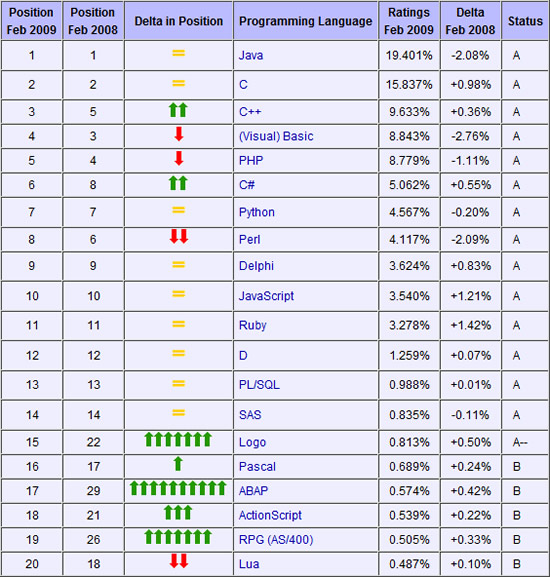
\includegraphics[width=\textwidth]{figuras/ranking}
    \fonte{o autor.}
\end{quadro}

% ----------------- Gráfico ------------- %
%O Gráfico \ref{fig:grafico2} foi criado utilizando o ambiente "grafico".
\begin{grafico}[!htpb]
 \centering
	\caption{Exemplo de gráfico}
	\label{graf:grafico2}
 	\borda{
 		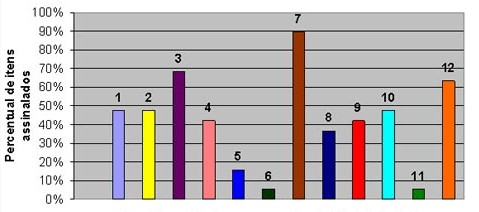
\includegraphics[scale=0.4]{figuras/grafico}
    }
    \fonte{o autor.}
\end{grafico}



% ----------------- Fotografia ------------- %
%A Fotografia \ref{fig:grafico3} foi criado utilizando o ambiente "fotografia".
\begin{fotografia}[!htpb]
 \centering
	\caption{Exemplo de fotografia}
	\label{fot:grafico3}
 	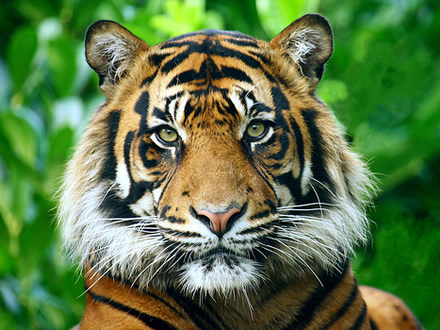
\includegraphics[width=\textwidth]{figuras/fotografia}
    \fonte{o autor.}
\end{fotografia}

% ----------------- Fluxograma ------------- %
%O Fluxograma \ref{fig:grafico4} foi criado utilizando o ambiente "fluxograma".
\begin{fluxograma}[!htpb]
 \centering
	\caption{Exemplo de fluxograma}
	\label{flux:grafico4}
	\borda{
 		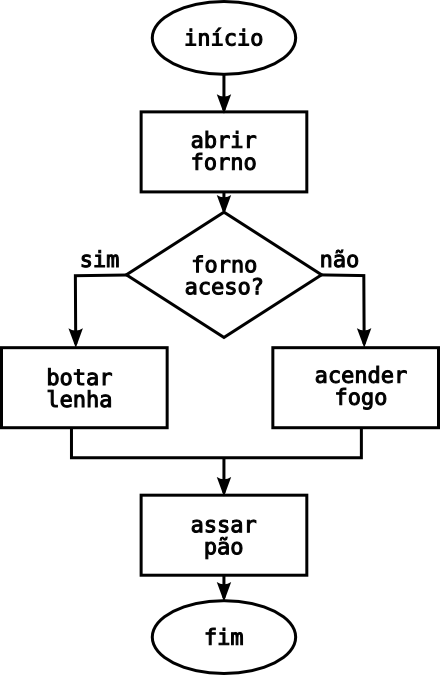
\includegraphics[scale=0.5]{figuras/fluxograma}
    }
    \fonte{o autor.}
\end{fluxograma}



% ----------------- Organograma ------------- %
%O Organograma \ref{fig:grafico5} foi criado utilizando o ambiente "orgonograma".
\begin{organograma}[!htpb]
 \centering
	\caption{Exemplo de organograma}
	\label{orga:grafico5}
	\borda{
 	  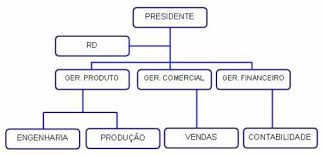
\includegraphics[scale=0.5]{figuras/organograma}
    }
    \fonte{o autor.}
\end{organograma}
% ----------------- Diagrama ------------- %
%O Diagrama \ref{fig:grafico6} foi criado utilizando o ambiente "diagrama".
\begin{diagrama}[!htpb]
 \centering
	\caption{Exemplo de diagrama}
	\label{diag:grafico6}
	\borda{
 	 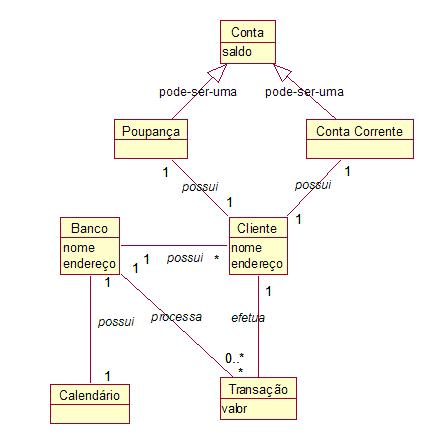
\includegraphics[scale=0.3]{figuras/diagrama}
    }
    \fonte{o autor.}
\end{diagrama}

% ----------------- Mapa ------------- %
%O Mapa \ref{fig:grafico7} foi criado utilizando o ambiente "mapa".
\begin{mapa}[!htpb]
 \centering
	\caption{Exemplo de mapa}
	\label{map:grafico7}
 	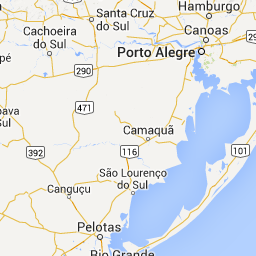
\includegraphics[scale=0.5]{figuras/mapa}
    \fonte{o autor.}
\end{mapa}

% ----------------- Esquema ------------- %
%O Esquema \ref{fig:grafico10} foi criado utilizando o ambiente "esquema".
\begin{esquema}[!htpb]
 \centering
	\caption{Exemplo de esquema}
	\label{esq:grafico10}
	\borda{
 		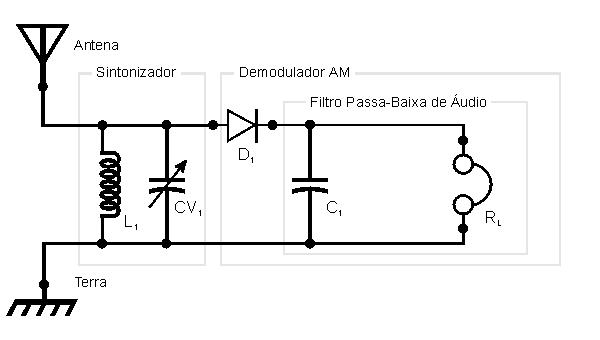
\includegraphics[scale=0.3]{figuras/esquema}
    }
    \fonte{o autor.}
\end{esquema}

% ----------------- Desenho ------------- %
%O Desenho \ref{fig:grafico9} foi criado utilizando o ambiente "desenho".
\begin{desenho}[!htpb]
 \centering
	\caption{Exemplo de desenho}
	\label{des:grafico9}
	\borda{
 		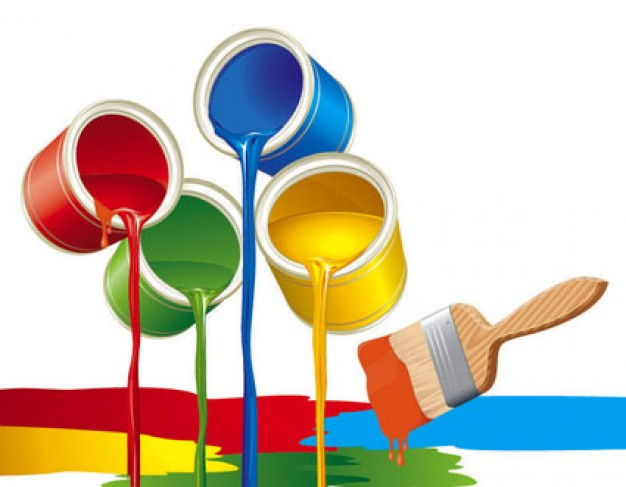
\includegraphics[scale=0.3]{figuras/desenho}
    }
    \fonte{o autor.}
\end{desenho}
\cleardoublepage

\section{CITAÇÃO}

Segundo  \citeonline[p. 94]{livro-unoesc},
\begin{citacao}
``Compreende trecho transcrito que apresenta mais de três linhas; mantém-se o discurso do texto original; destaca-se em blocos, espaço simples,com recuo de 4 cm a partir da margem esquerda, com letra menor que a do texto original;sugere-se usar tamanho 10''.
\end{citacao}

\section {LISTAS}
 Lorem ipsum dolor sit amet, consectetuer adipiscing elit. Ut purus elit, vestibulum ut, placerat ac, adipiscing vitae, felis. Curabitur dictum gravida mauris. Nam arcu libero, nonummy eget, consectetuer id, vulputate a, magna.

\begin{itemize}
\item Nam dui ligula, fringilla.
\item Nam dui ligula, fringilla.
\item Nam dui ligula, fringilla.
\end{itemize}

Lorem ipsum dolor sit amet, consectetuer adipiscing elit. Ut purus elit, vestibulum ut, placerat ac, adipiscing vitae, felis. Curabitur dictum gravida mauris. Nam arcu libero, nonummy eget, consectetuer id, vulputate a, magna.

\begin{enumerate}
 \item enumA
 \item enumB
\end{enumerate}

